\def\CC{{C\nolinebreak[4]\hspace{-.05em}\raisebox{.4ex}{\tiny\bf ++}}}

% TODO : NAME
% Copy, s/NAME/yourname/
%======================================================================
% lookup col 1 vs. col 2
\begin{frame}\frametitle{}
\vspace*{0.2in}
\centerline{\textrm{{\huge\bfseries\color{myOrange} State of \textit{MIRGE-Com}}}}
\smallskip
\centerline{\textrm{{\large\bfseries{Fri@CEESD - \today}}}}
%\centerline{\textrm{{\big\bfseries\color{myOrange} Anatomy of a large scale prediction}}}
\vspace*{0.2in}
%\hrule
%\begin{center}
%\includegraphics[width=0.85\textwidth]{Figures/TitleFig.pdf}
%\end{center}
%\hrule
\begin{center}
\vspace*{0.4in}
\cPI{Mike Campbell}
\end{center}
\end{frame}

\begin{frame}\frametitle{Overview}
\vspace*{0.1in}
\bfseries{\color{myOrange} Goal}:\\
Get started with \textit{MIRGE-Com}; know where to look, or who to ask for help.\\
\vspace{0.2in}
\bfseries{\color{myOrange} Outline}:\\
\begin{multicols}{2}
\begin{itemize}
  \item Overview - the general idea
  \item Current state - team, code, how to get, install, package tour
  \item Example application: Euler flow solver
  \item Demo
  \item Next steps
  %   \begin{itemize}
  %      \item like JBF/AK, full architecture
  %       \item limited view
  %  \end{itemize}      
  %  \item Development team
  %  \item Getting mirgecom
  %  \begin{itemize}
  %    \item Documentation
  %    \item Installation
  %  \end{itemize}
%  \item Using mirgecom
%  \begin{itemize}
%    \item How to get your grid into mirgecom
%    \item Visualization
%    \item Evolution equations: Euler
%    \begin{itemize}
%      \item Inviscid operator for RHS
%      \item LaxFriedrichs flux
%      \item EOS
%      \item BoundaryConditions
%      \item RK4
%      \item SimUtils
%      \item Example (demo + driver review)
%    \end{itemize}
%  \end{itemize}
%  \item Big todos
%  \begin{itemize}
%    \item Restart
%    \item Navier-Stokes
%    \item Chemistry
%    \item Performance, scaling and modeling, CPU, GPU,, PC2
%  \end{itemize}
\end{itemize}
\end{multicols}
\end{frame}

%\begin{frame}\frametitle{Integrating \textit{Prometheus} into \textit{MIRGE-Com}}
%Main components to consider for integration:
%\begin{multicols}{2}
%\begin{itemize}
%  \item Code generator
%  \begin{itemize}
%    \item \plusplus{C} command-line utility 
%    \item XML $\rightarrow$ \textit{Prometheus}(\textit{Cantera}) $\rightarrow$ Python API 
%  \end{itemize}
%  \item Mixture API
%  \item Physics
%  \begin{itemize}
%    \item Thermodynamics (mixture EOS)
%    \item Chemistry (species production rates)
%    \item Transport (``advanced'' \& mixture-averaged properties)
%  \end{itemize}
%\item \textit{Cantera} TPL
%\end{itemize}
%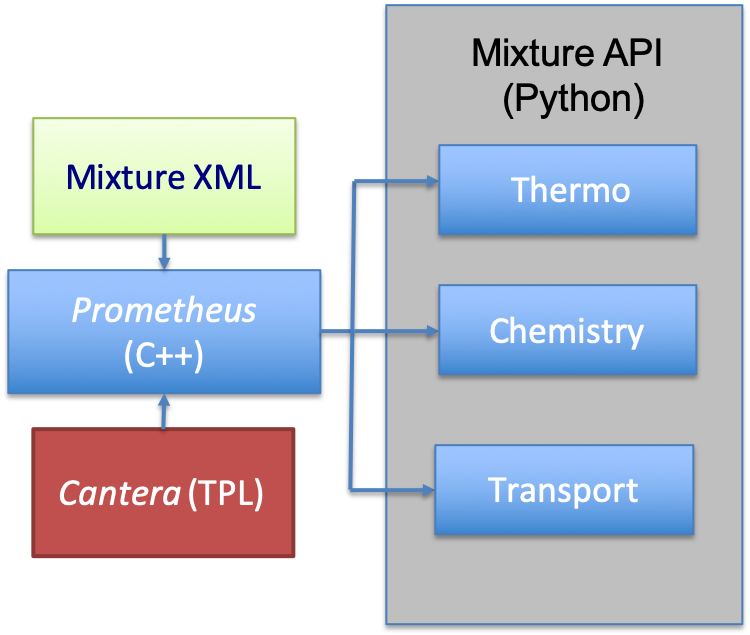
\includegraphics[width=.5\textwidth]{figures/prometheus_cartoon.png}
%\end{multicols}
%\end{frame}

\begin{frame}\frametitle{MIRGE Overview}
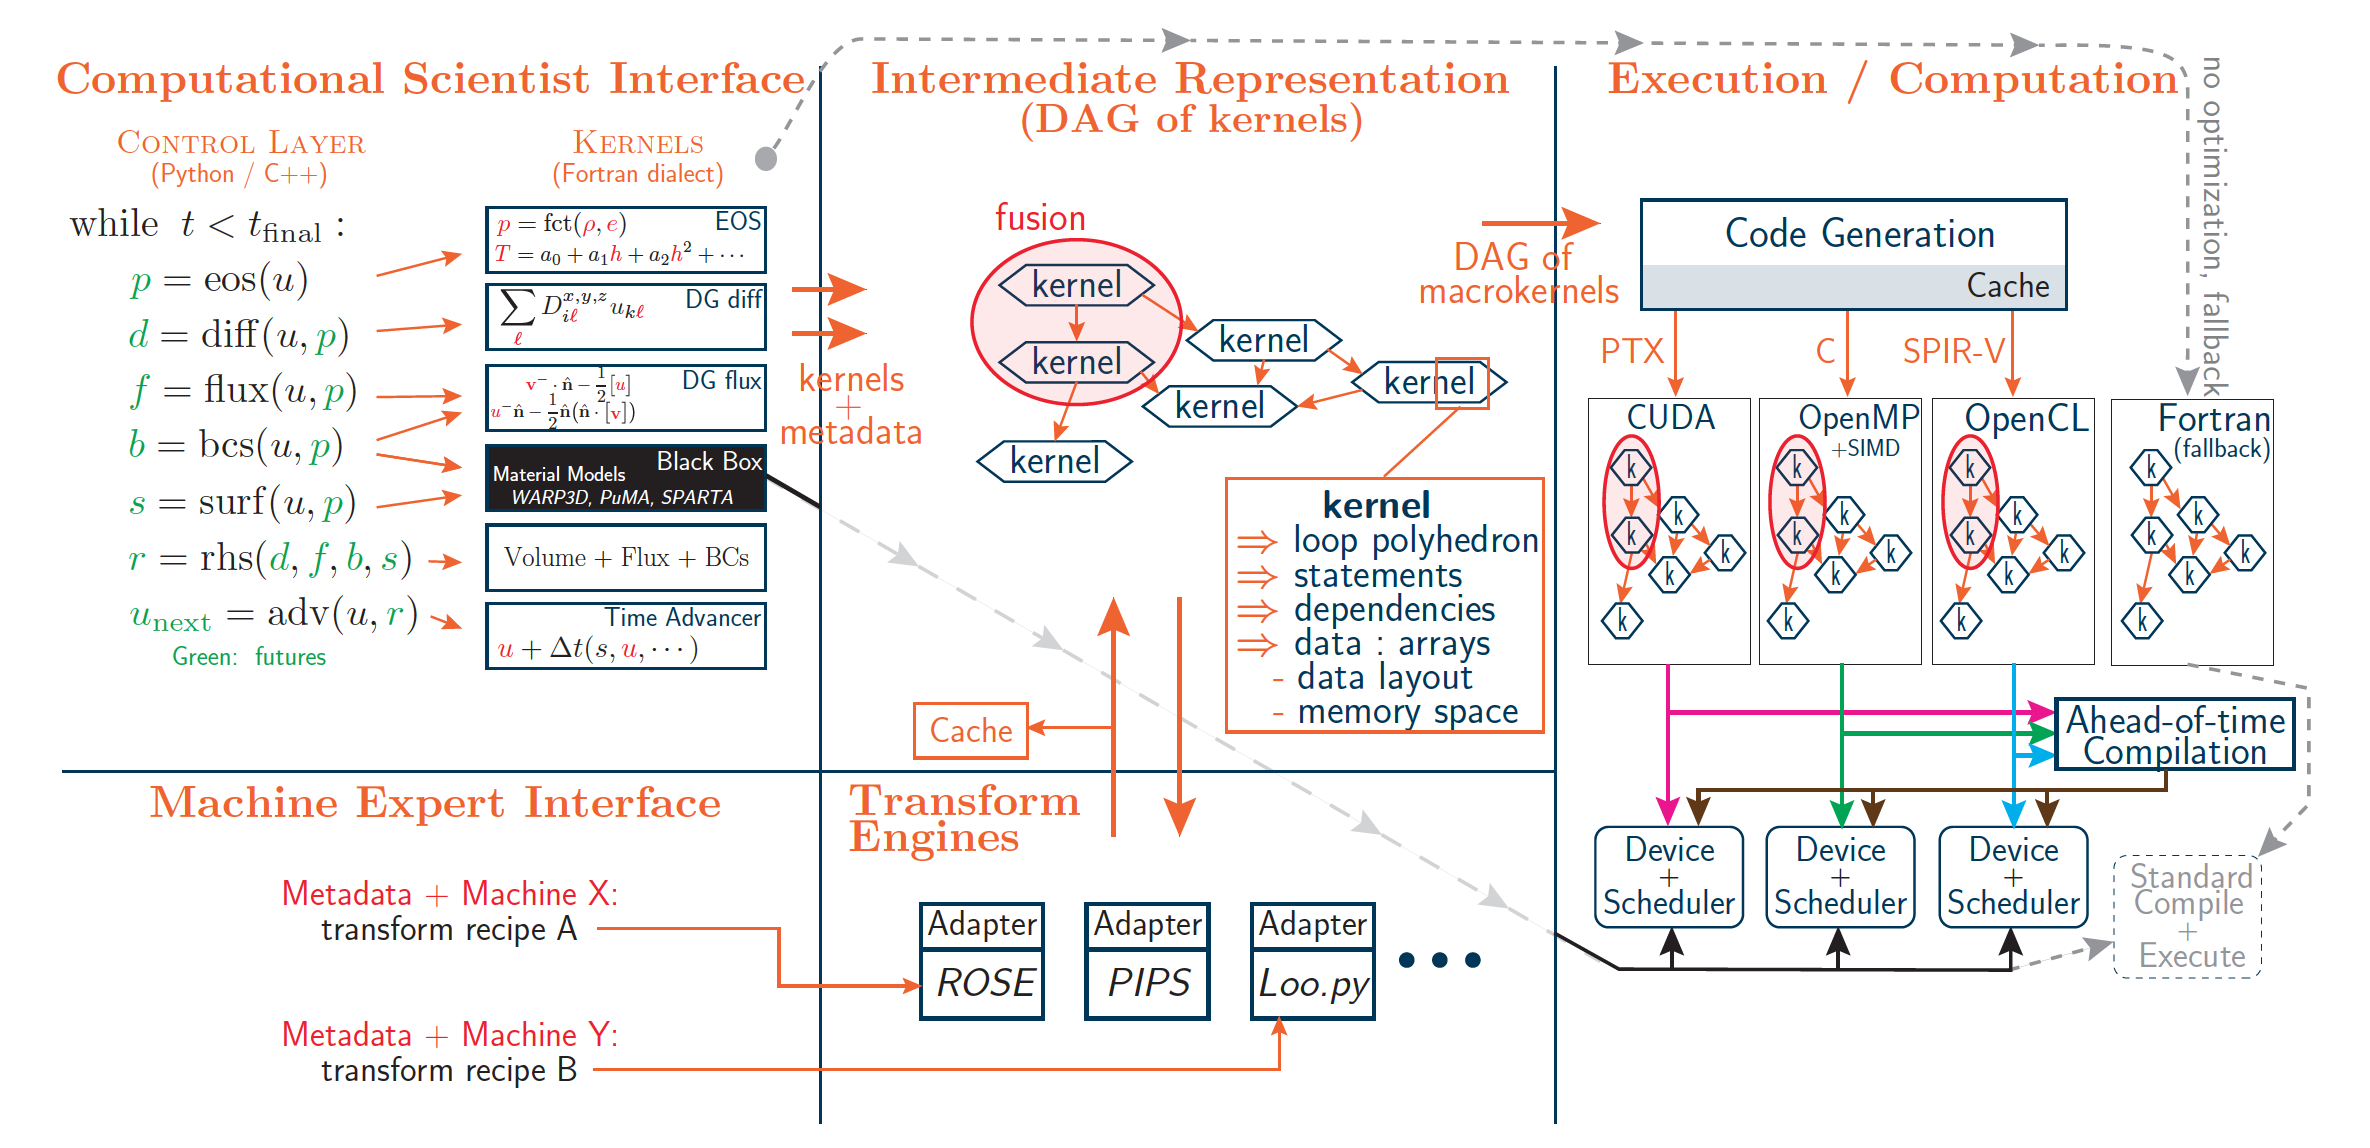
\includegraphics[width=\textwidth]{figures/MIRGE.png}
\begin{center}
[Kl{\"o}ckner]
\end{center}
\end{frame}

\begin{frame}\frametitle{Development team}
\begin{multicols}{2}
\begin{itemize}
\item Mike Anderson - predictions, modeling
\item Mike Campbell - sim/solver development
\columnbreak
\item Matthias Diener - environment, platforms, performance
\item Matt Smith  - sim/solver development, grids/geometry
\end{itemize}
\end{multicols}
\end{frame}

% official faculty ref. by name?
\begin{frame}\frametitle{About \textit{MIRGE-Com}}
\begin{multicols}{2}
\begin{itemize}
  \item \textit{MIRGE-Com}: API for building MIRGE simulation applications
  \item CEESD community code: \href{https://github.com/illinois-ceesd/mirgecom}{(\textcolor{blue}{https://github.com/illinois-ceesd/mirgecom})}
  \item Builds on several pre-existing packages; most notably Kl{\"o}ckner's suite of Python tools
  \item Users' interface for engaging CEESD MIRGE machinery to run on modern platforms
\end{itemize}
\end{multicols}
\begin{multicols}{2}
%\begin{center}
\hspace{.6in}
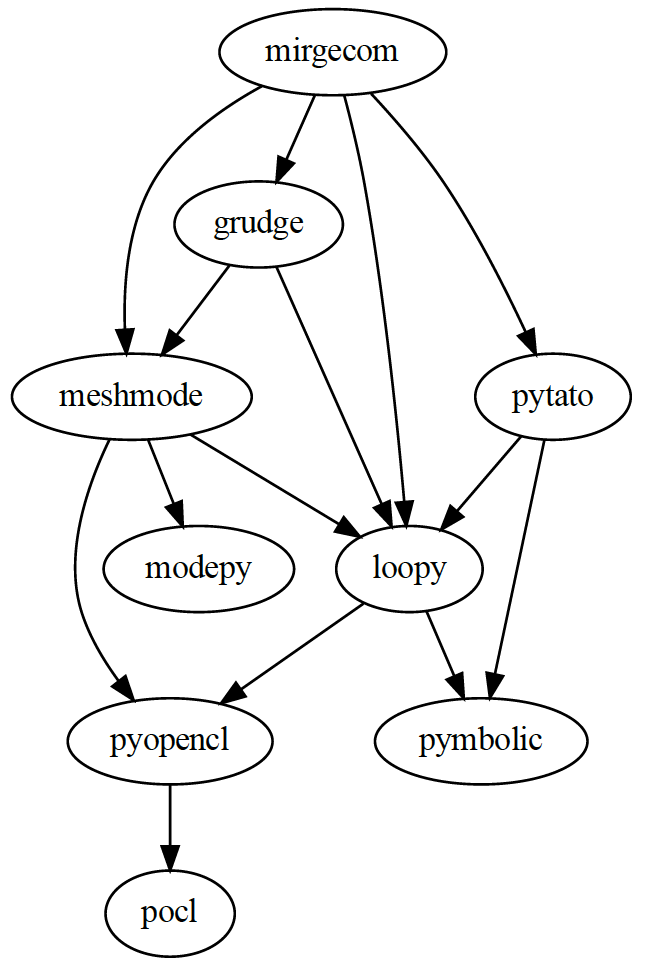
\includegraphics[width=.25\textwidth]{figures/MirgecomPackageTree.png}
\hspace{-.4in}
\vspace{-.2in}
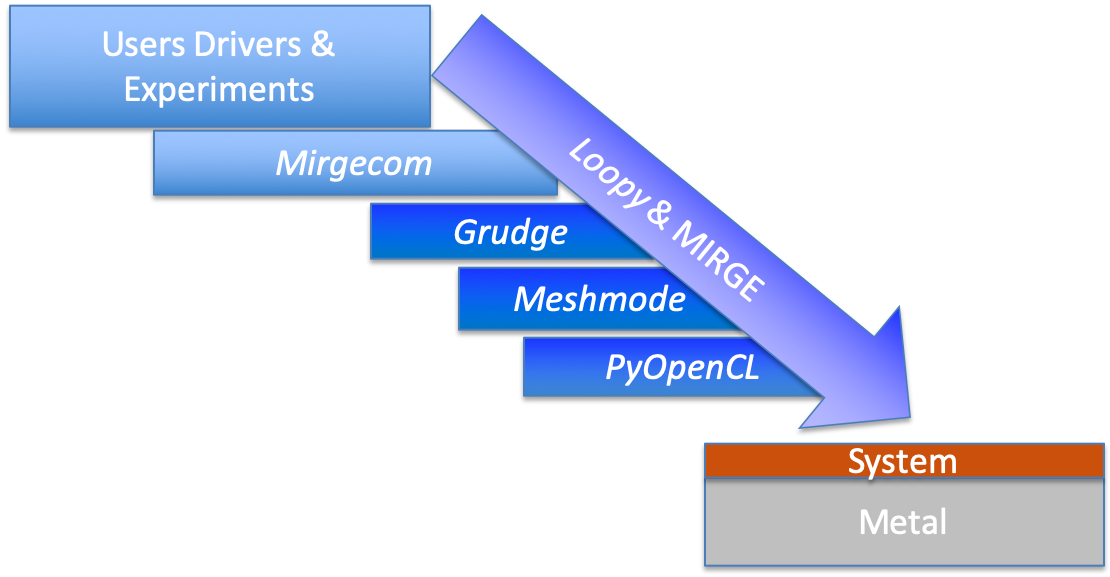
\includegraphics[width=.5\textwidth]{figures/mirgecom_cartoon.png}
\end{multicols}
%\end{center}
\end{frame}

\begin{frame}\frametitle{Core packages}
\begin{itemize}
  \item Loo.py (\href{https://github.com/inducer/loopy}{(\textcolor{blue}{https://github.com/inducer/loopy})})
  \begin{itemize}
    \item Code generator and transform tool
    \item IR in MIRGE
    \item Element-wise computational kernels
  \end{itemize}
  \item Meshmode (\href{https://github.com/inducer/meshmode}{(\textcolor{blue}{https://github.com/inducer/meshmode})})
  \begin{itemize}
    \item Uns., high-order, discont. piecewise polynomial discretizations 
    \item DG building blocks (see \texttt{examples/simple-dg.py}).
  \end{itemize}
  \item \textit{Grudge} - 1/2/3D DG based on \textit{meshmode} (\href{https://github.com/inducer/grudge}{(\textcolor{blue}{https://github.com/inducer/grudge})})
  \begin{itemize}
    \item Multiple \textit{meshmode} discretizations
    \item Methods and operations - math, projections, norms and reductions
  \end{itemize}
\end{itemize}
\end{frame}

\begin{frame}\frametitle{Getting started with \textit{MIRGE-Com}}
\begin{multicols}{2}
\begin{itemize}
  \item \textit{Emirge} - \textit{MIRGE-Com} installation tool
  \begin{itemize}
    \item > git clone https://github.com/illinois-ceesd/emirge
    \item > install.sh
    \item > source config/activate\_env.sh
  \end{itemize}
  \item \textit{MIRGE-Com} documentation
  \begin{itemize}
    \item > conda install sphinx
    \item > cd mirgecom/doc \&\& make html
  \end{itemize}
\end{itemize}
%\hspace{.8in}
%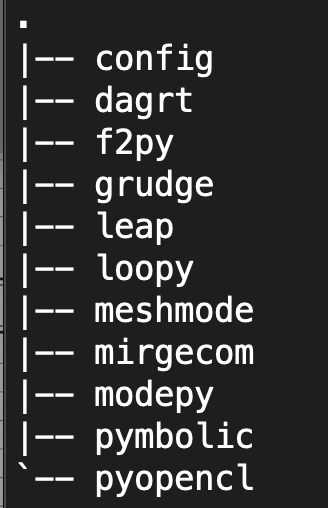
\includegraphics[width=.2\textwidth]{figures/emirge_dirs.png}
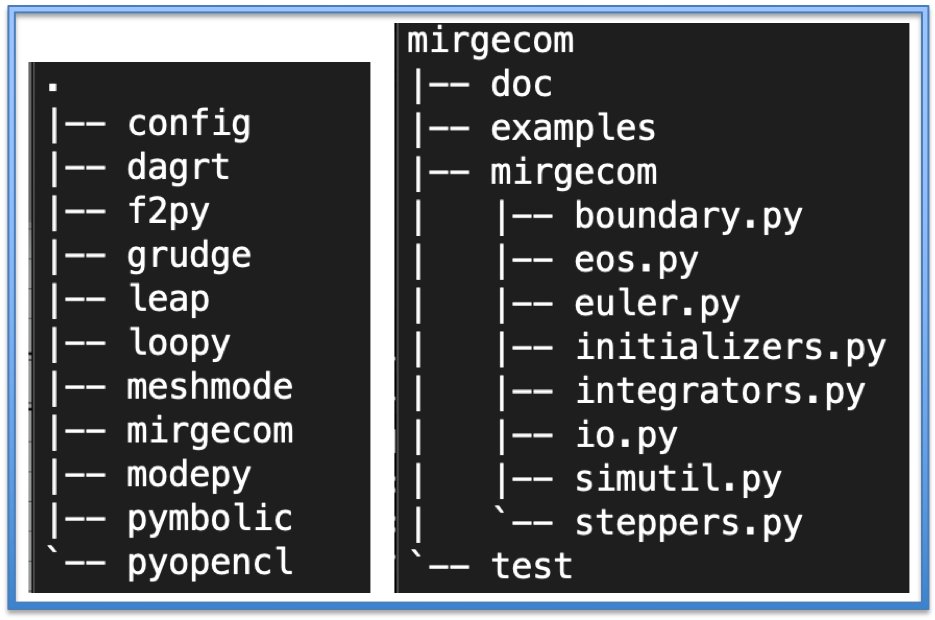
\includegraphics[width=.5\textwidth]{figures/dir_trees.png}
\end{multicols}
\begin{center}
\href{https://github.com/illinois-ceesd/emirge}{(\textcolor{blue}{https://github.com/illinois-ceesd/emirge})}
\href{https://mirgecom.readthedocs.io/en/latest/}{(\textcolor{blue}{https://mirgecom.readthedocs.io/en/latest/})}
\end{center}
\end{frame}

\begin{frame}\frametitle{\textit{MIRGE-Com} use case: Euler}
\begin{center}
Evolution equation:
\begin{equation}
  \frac{\partial\mathbf{Q}}{\partial{t}} = - (\nabla \cdot \mathbf{F})
\end{equation}
Where state vector $\mathbf{Q}$, and the inviscid fluxes $\mathbf{F}$ are given by:
\begin{equation}
%\begin{align}
\mathbf{Q} = \begin{bmatrix} \rho\\\rho{E}\\\rho\vec{v}\\\rho{Y}_\alpha\end{bmatrix}, \mathbf{F} = \begin{bmatrix} \rho\vec{v}\\(\rho{E} + p)\vec{v}\\\rho(\vec{v} \otimes \vec{v}) + p\delta_{ij}\\\rho{Y}_\alpha\vec{v}\end{bmatrix}
%\end{align}
\end{equation}
\begin{itemize}
\item Core implementation in \texttt{mirgecom/euler.py}
\end{itemize}
%\begin{center}
(\href{https://doi.org/10.1007/978-0-387-72067-8}{\textcolor{blue}{Hesthaven and Warburton, Nodal DG Methods}})\\
(\href{https://mirgecom.readthedocs.io/en/latest/operators.html}{\textcolor{blue}{https://mirgecom.readthedocs.io/en/latest/operators.html}})\\
\end{center}
\end{frame}
%
%
\begin{frame}\frametitle{State vector handling}
\begin{multicols}{2}
\begin{itemize}
  \item State vector handling in \texttt{euler.py}
  \item Grid supported data arrays underpinned by \textit{meshmode} DOFArray:
  \begin{itemize}
    \item is an object array of numpy-compatible arrays (\#DOF x \#Elements *of a given type*)
    \item has an array context - hook for device, transformations, etc
    \item \textit{Grudge} DGDiscretization (and Eager equivalent)  provides encapsulation for discretizations with multiple element types, subdiscretizations
  \end{itemize}
  \item Dataclass: ConservedVariables for convenience
  \item Hides data layout (none of my business)
  \item Developers focus on content
\end{itemize}
\end{multicols}
\begin{center}
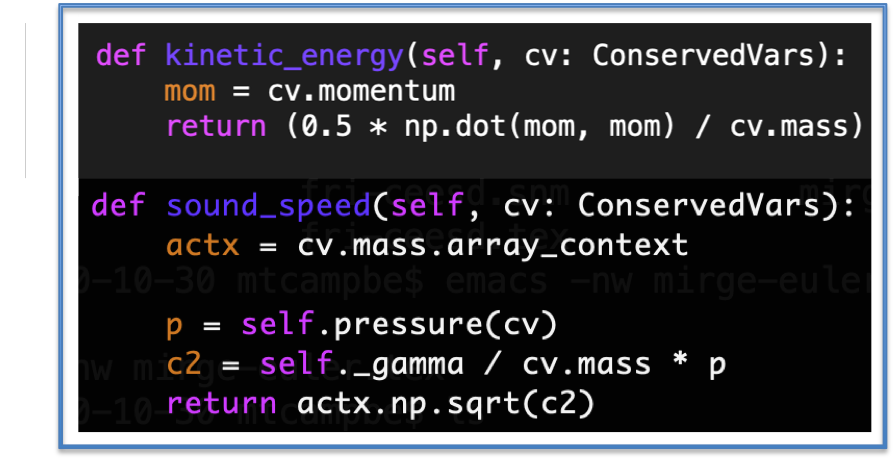
\includegraphics[width=.5\textwidth]{figures/eos_sample.png}
\end{center}
\end{frame}


\begin{frame}\frametitle{Inviscid flux implementation}
$\mathbf{F} = \langle\rho\vec{v}, (\rho{E} + p)\vec{v}, \rho(\vec{v}\otimes\vec{v}) + p\mathbf{I}\rangle$
\begin{center}
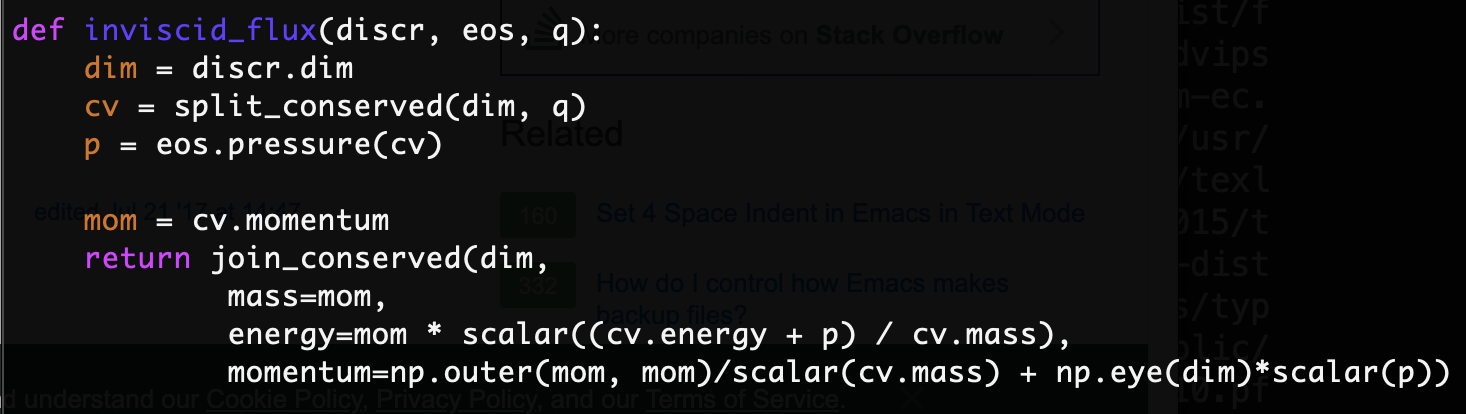
\includegraphics[width=\textwidth]{figures/inviscid_flux.png}
\end{center}
\begin{itemize}
  \item Code expression is very close to the math.
  \item CV data handling construct works for vectors
\end{itemize}
\end{frame}

\begin{frame}\frametitle{Facial fluxes - element boundary}
Local Lax-Friedrichs flux:
$\mathbf{F}^* = \{\{\mathbf{F}\}\}\cdot\hat{\mathbf{n}} + \frac{\lambda}{2}[[\mathbf{Q}]]$
\begin{center}
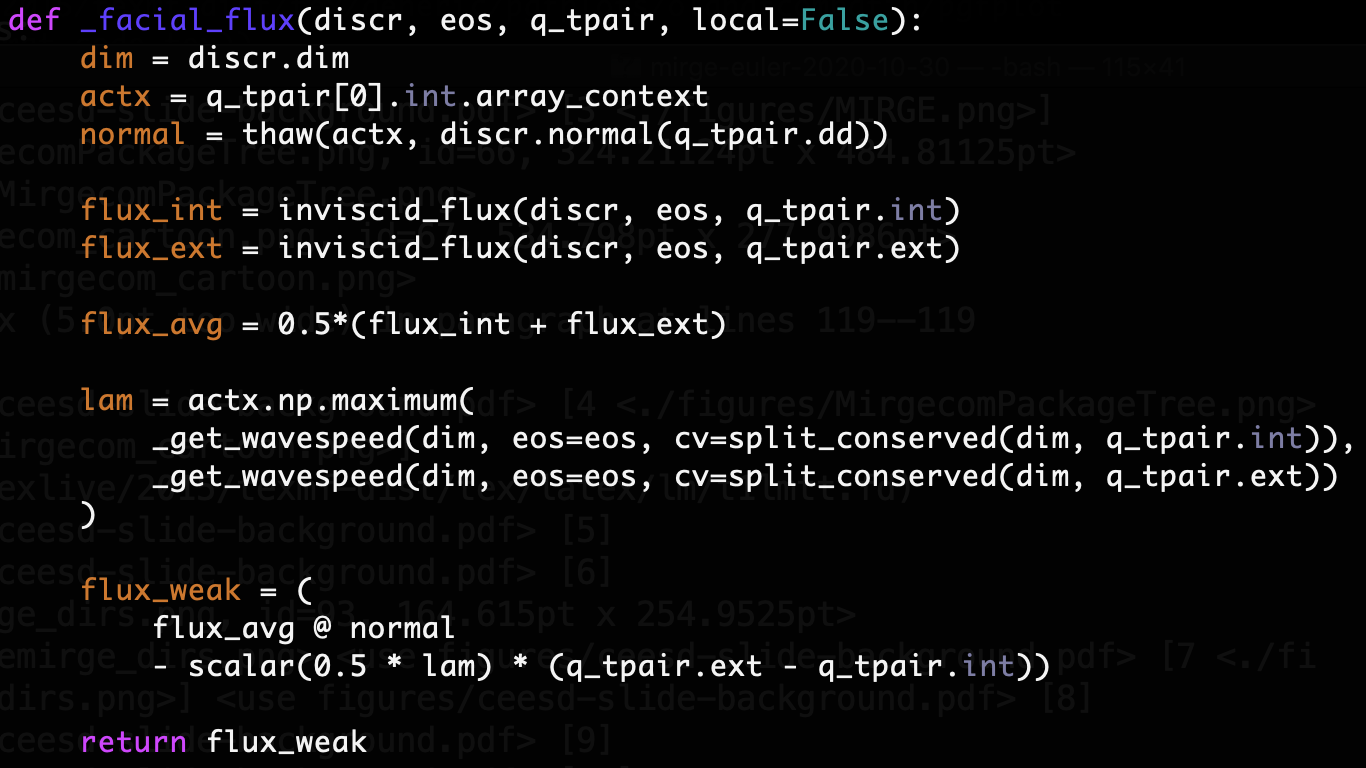
\includegraphics[width=.8\textwidth]{figures/facial_flux.png}
\end{center}
$\{\{\mathbf{F}\}\} = \frac{(\mathbf{F}^{+} + \mathbf{F}^{-})}{2}, [[\mathbf{Q}]] = (\mathbf{Q}^{-} - \mathbf{Q}^{+})\cdot\hat{\mathbf{n}}$
\begin{itemize}
\item \textit{Grudge} TracePair encapsulation for int/ext (-/+) facial pairs.
\end{itemize}
\end{frame}

\begin{frame}\frametitle{Boundary conditions}
\begin{itemize}
  \item BC implementations in \texttt{mirgecom/boundary.py}
  \item Returns \textit{Grudge} TracePair on boundary traces
  \item \textit{Grudge} DGDiscretization \textbf{project} data between DOFDesc (dd, sub-discretizations)
\end{itemize}
\begin{center}
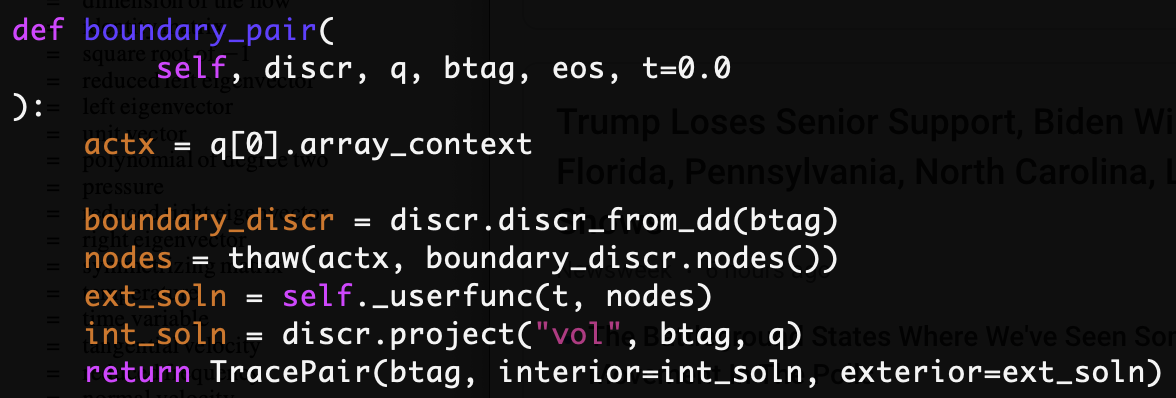
\includegraphics[width=.8\textwidth]{figures/boundary_condition.png}
\end{center}
\end{frame}


\begin{frame}\frametitle{Euler RHS}
\begin{multicols}{2}
\begin{itemize}
  \item \textit{Grudge} DGDiscretization provides:
  \begin{itemize}
    \item divergence operator
    \item interior\_trace\_pair - selects all interior faces
    \item cross\_rank\_trace\_pairs - selects all partition boundary pairs
    \item mass matrices
  \end{itemize}
  \item User provides:
  \begin{itemize}
    \item boundaries
    \item EOS (\texttt{mirgecom/eos.py})
    \item $\mathbf{Q}$
    \item flux routines
  \end{itemize}
\end{itemize}
\columnbreak
\hspace{-.2in}
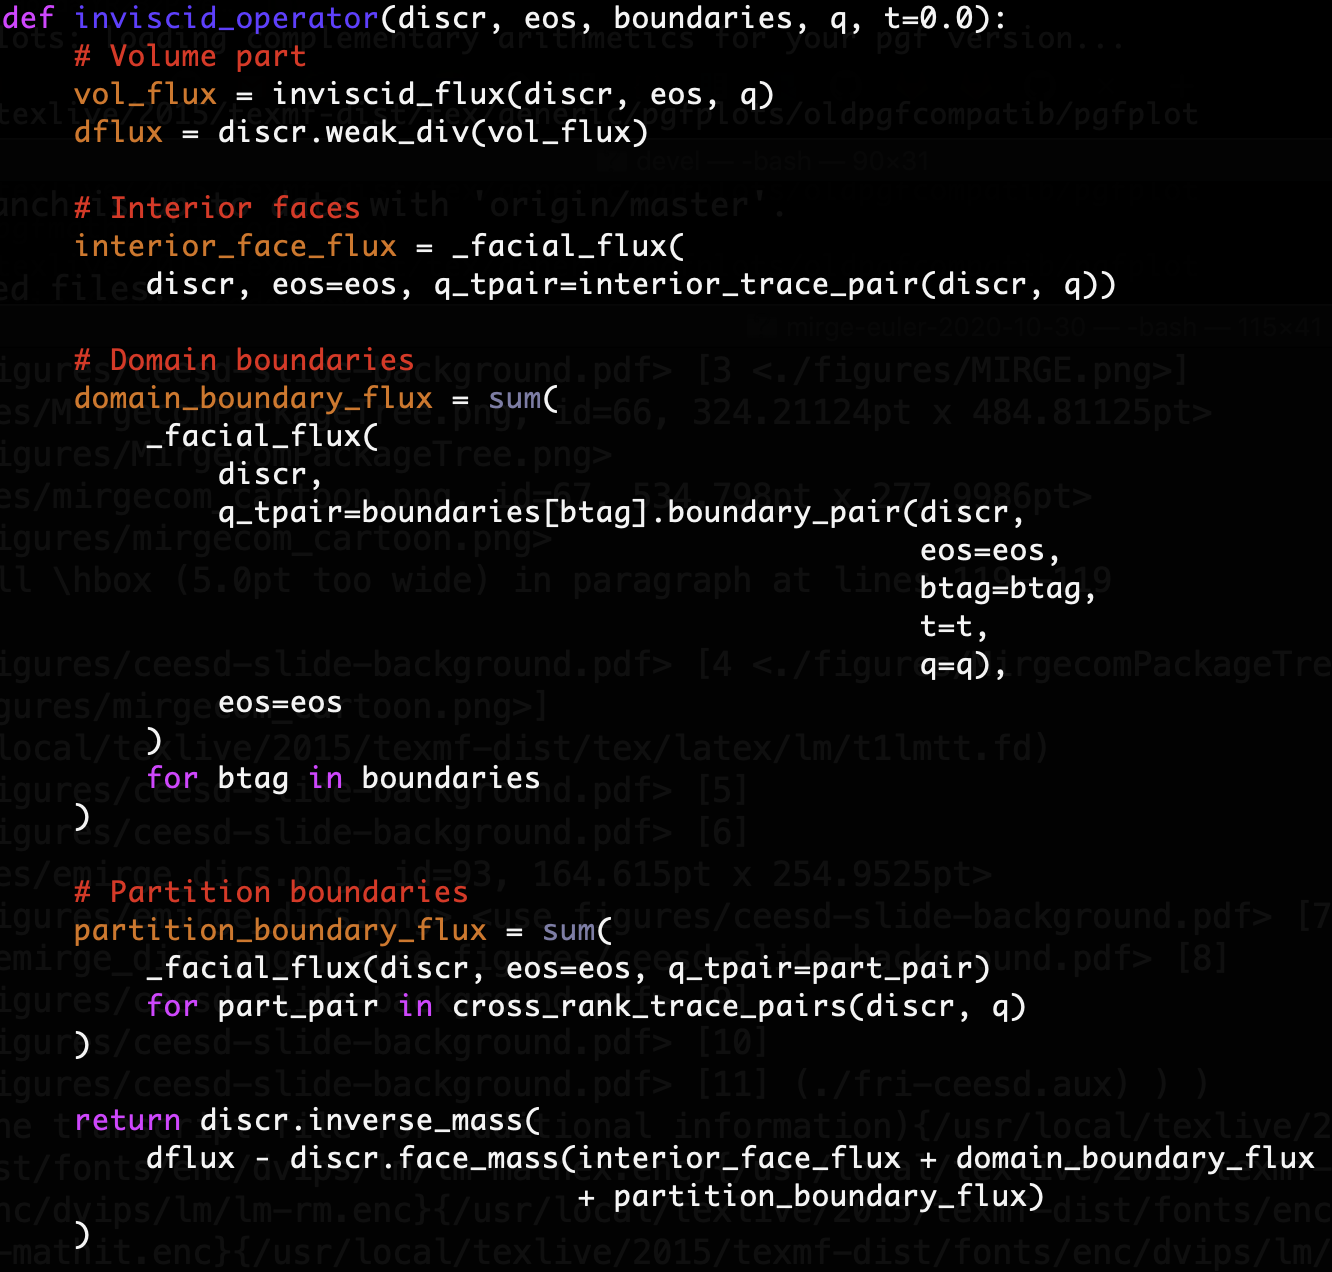
\includegraphics[width=.6\textwidth]{figures/inviscid_operator.png}
\end{multicols}
\end{frame}

\begin{frame}\frametitle{Example Euler simulation application}
\begin{multicols}{2}
\begin{itemize}
\item Isentropic vortex example (and others) - \texttt{examples/vortex-mpi.py}
\item Solution initialization (\texttt{mirgecom/initializers.py})
\item Generic timestepping (\texttt{mirgecom/steppers.py})
\item RK4 time integrator (\texttt{mirgecom/integrators.py})
\item Exact soln comparison, checkpointing (\texttt{mirgecom/simutil.py})
\item Screen and viz I/O (\texttt{mirgecom/io.py})
\end{itemize}
\end{multicols}
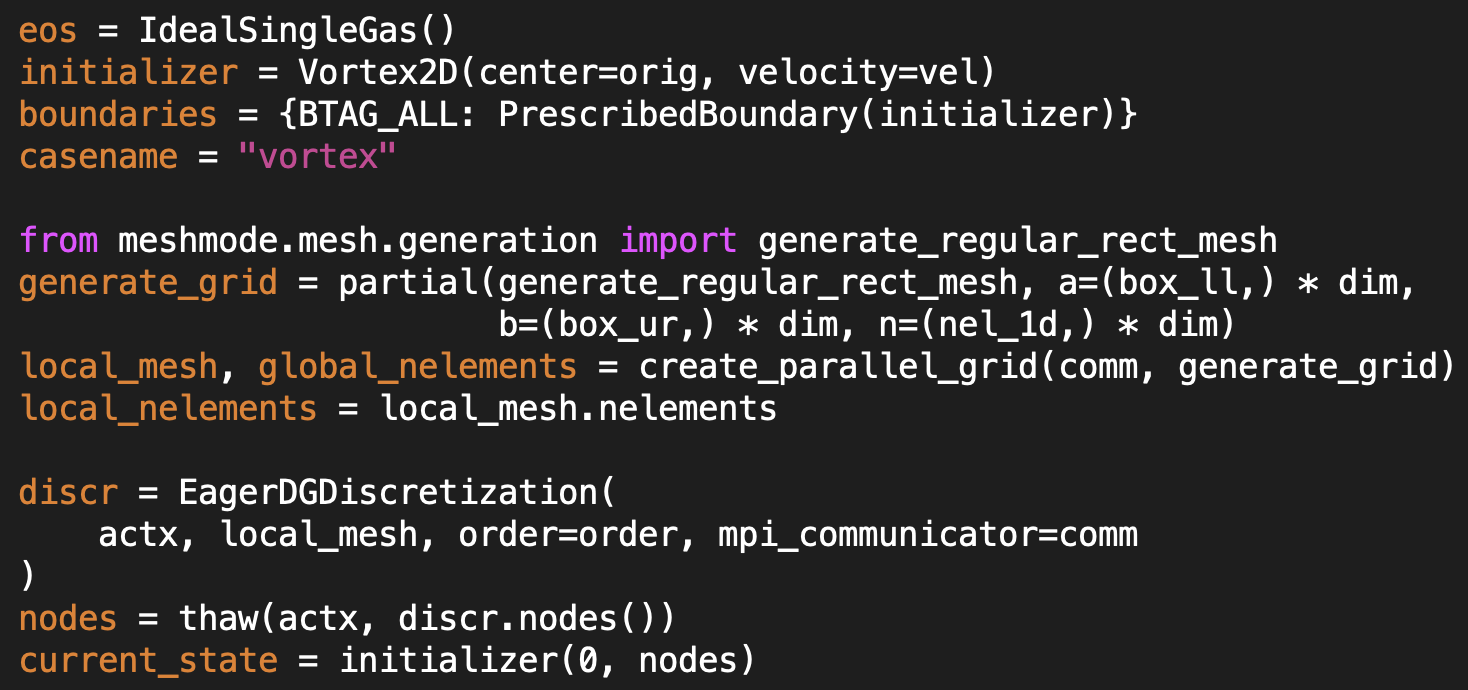
\includegraphics[width=.45\textwidth]{figures/vortex_driver1.png}
\hspace{.2in}
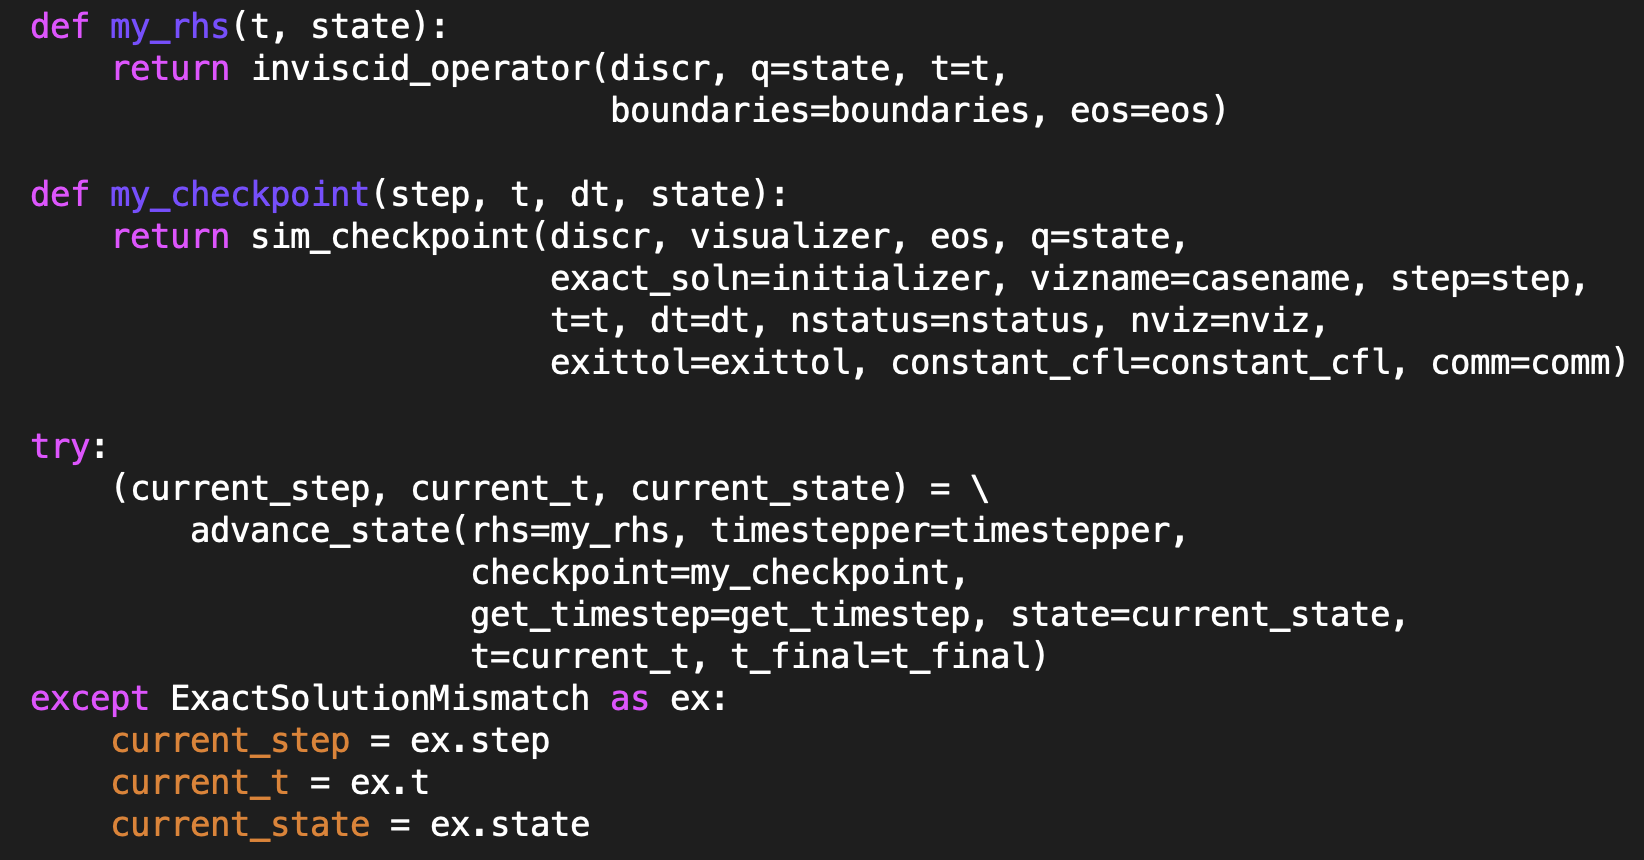
\includegraphics[width=.45\textwidth]{figures/vortex_driver2.png}
\end{frame}
%\begin{frame}\frametitle{Plan for \textit{Prometheus} code generation}
%\begin{multicols}{2}
%\begin{itemize}
%  \item Port \textit{Prometheus} to Python
%  \item User provides mixture XML input
%  \item \textit{Mirgecom} interfaces \textit{Prometheus} Python package to generate mixture API inline
%  \item \textit{Prometheus} Python package depends on \textit{Cantera}
%  \item Question: Wrap generated API, or directly generate \textit{mirgecom} EOS, chemistry, transport?
%\end{itemize}
%\end{multicols}
%\begin{center}
%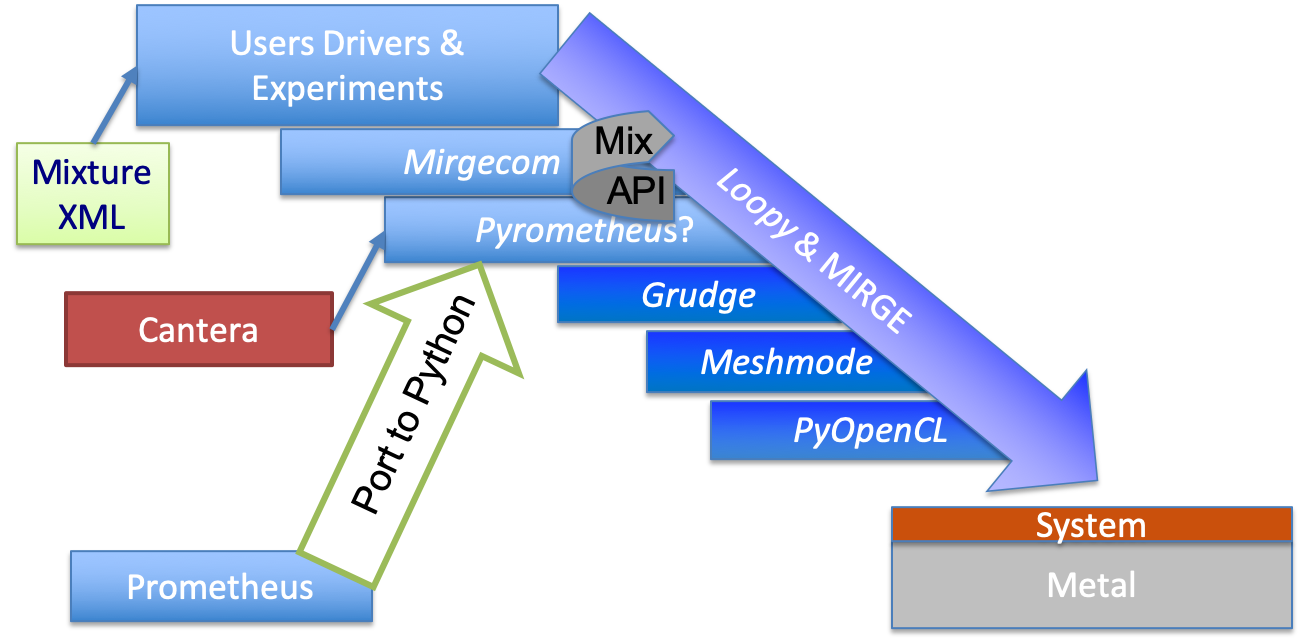
\includegraphics[width=.8\textwidth]{figures/ultimate_integration.png}
%\end{center}
%\end{frame}

%\begin{frame}\frametitle{Planning for the plan - partial integration}
%\begin{multicols}{2}
%\begin{itemize}
%  \item Use \textit{Prometheus} as-is, generate Mixture API to file 
%  \item Use Mixture API directly in \textit{mirgecom}
%  \item Useful for testing and development of \textit{mirgecom} components that use Mixture API (regardless o%f source)
%  \item Far less convenient to use (from user's perspective)
%\end{itemize}
%\end{multicols}
%\begin{center}
%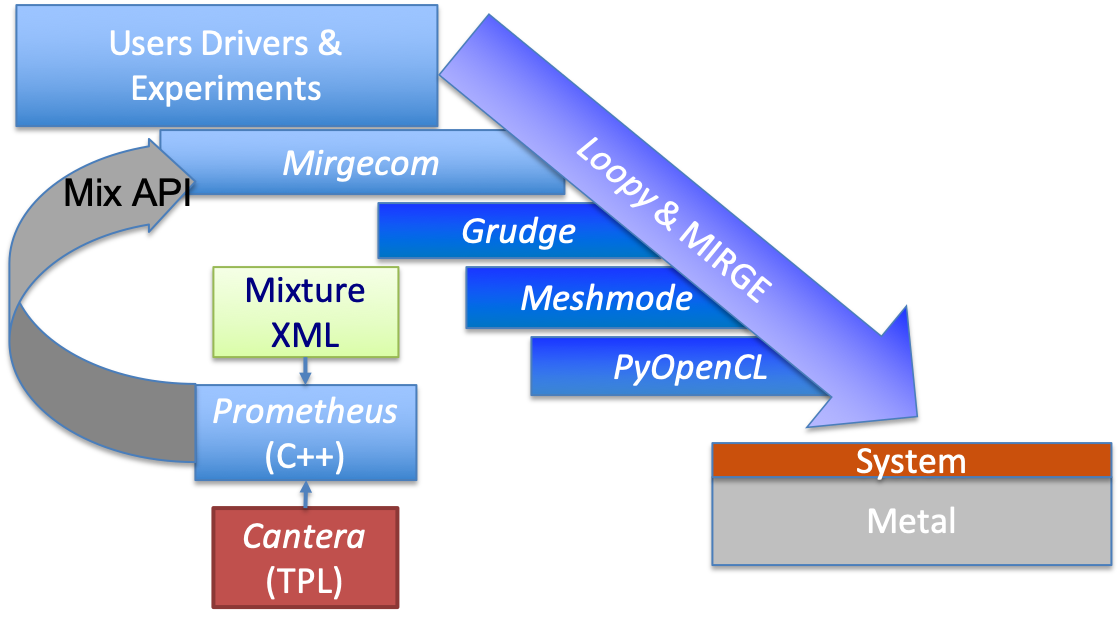
\includegraphics[width=.8\textwidth]{figures/partial_cartoon.png}
%\end{center}
%\end{frame}

%\begin{frame}\frametitle{Evolution equations for \textit{mirgecom}}
%\begin{center}
%(\href{https://mirgecom.readthedocs.io/en/latest/operators.html}{\textcolor{blue}{https://mirgecom.readthedocs.io/en/latest/operators.html}})\\
%Governing equations for compressible, reactive flow:
%\begin{equation}
%  \frac{\partial\mathbf{Q}}{\partial{t}} = \mathbf{S} - (\nabla \cdot \mathbf{F}^I) + (\nabla \cdot \mathbf{F}^V)
%\end{equation}
%Where $\mathbf{Q} = [\rho, \rho{E}, \rho\vec{V}, \rho{Y}_\alpha]$, and the inviscid, viscous flux, and source vectors are given by:
%\begin{equation}
%\begin{align}
%\mathbf{F}^I = \begin{bmatrix} \rho\vec{V}\\(\rho{E} + p)\vec{V}\\\rho(\vec{V} \otimes \vec{V}) + p\delta_{ij}\\\rho{Y}_\alpha\vec{V}\end{bmatrix}, \mathbf{F}^V = \begin{bmatrix}0\\\mathbf{\tau}\cdot\vec{V} - \vec{q}\\\mathbf{\tau}\\\phi_\alpha\end{bmatrix}, \mathbf{S} = \begin{bmatrix}0\\0\\0\\W_\alpha\dot{\omega}_\alpha\end{bmatrix}
%\end{align}
%\end{equation}
%\textit{mirgecom} currently implements only $\mathbf{F}^I$ in the Euler module, with $\mathbf{S}$ trivially added.
%\end{center}
%\end{frame}
%\begin{frame}\frametitle(Integrating \textit{Prometheus} code generator}
%\begin{multicols}{2}
%\begin{itemize}
%   \item Integration options:
%   \begin{itemize}
%      \item Full integration - \textit{mirgecom} ingests XML, uses \textit{Prometheus} to generate mechanism, %including mechanism in \textit{mirgecom} library
%      \item Partial integration - \textit{Prometheus} pre-generates mechanism for inclusion of interface into %\textit{mirgecom} library
%      \item Non-integration - \textit{Prometheus} stand-alone library implements one or more mechanisms and is% used as a substrate library by \textit{mirgecom} 
%   \end{itemize}
%    \item Staged integration - partial $\rightarrow$ full
%   \item Tests we can do right away (regardless of integration level):
%   \begin{itemize}
%      \item Pre-generated mechanism Python code inclusion (\textit{mirgecom} build and run)
%      \item Pre-generated mechanism function invocations (smoke tests \& screening)
%   \end{itemize}
%\end{itemize}
%\end{multicols}
%\end{frame}

%\begin{frame}\frametitle{\textit{Prometheus} Mixture API $\rightarrow$ \textit{mirgecom} EOS}
%\begin{center}
%  \textit{Mirgecom} EOS interface (\href{https://mirgecom.readthedocs.io/en/latest/operators.html\#equations-of-state}{\textcolor{blue}{https://mirgecom.readthedocs.io/en/latest/operators.html\#equations\-of\-state}})
%\end{center}
%\begin{multicols}{2}
%\begin{itemize}
%  \item Inviscid setting - EOS used for pressure terms in $\mathbf{F}^I$, soln initialization, boundary conditions
%  \item \textit{Prometheus} Mixture API thermo properties functions:
%  \begin{itemize}
%    \item Mixture properties: $(e, T, p, Cp, R, h)$
%    \item Species properties: $(h_\alpha, Cp_\alpha, R_\alpha)$
%    % \item get\_temperature(e, Y, Tguess) $\rightarrow (T, Cp_{mix}, R_{mix})$
%    % \item get\_pressure(Y, T) $\rightarrow P_{mix}$ 
%    % \item get\_mix\_cp(T, Y) $\rightarrow (Cp_{mix})$ 
%    % \item get\_mix\_cv(T, Y) $\rightarrow (Cv_{mix})$
%    % \item get\_mix\_e(T, Y) $\rightarrow (e)$
%    % \item get\_mix\_enthalpy(T, Y) $\rightarrow (h_{mix})$
%    % \item ( ... )
%    % \item get\_species\_cp\_R(T) $\rightarrow (Cp_{i})$ 
%    % \item get\_species\_enthalpies(T, Y) $\rightarrow (h_{i})$
%  \end{itemize}
%  \item Plenty rich enough to implement \textit{mirgecom} mixture EOS:\\$P = (\gamma_{mix} - 1)\bar\rho{e}_{mix}$,\\ $T = \frac{(\gamma_{mix} - 1)}{R_{mix}} e_{mix}$
%   \item Special considerations
%   \begin{itemize}
%      \item Species ordering, naming
%      \item Buffer species handling
%   \end{itemize}
%   \item Potential tests in inviscid setting:
%   \begin{itemize}
%     \item Species-specific mixture tests (i.e. one species-at-a-time)
%     \item Calorically perfect mixture - Compare Prometheus vs. \textit{mirgecom}@CPEOS
%     \item Thermally perfect mixture with linear $Cp_i$ - test temperature inversion vs. analytic? 
%   \end{itemize}
%\end{itemize}
%\end{multicols}
%\end{frame}

%\begin{frame}\frametitle{Wrappers for \textit{Prometheus} EOS}
%Create \textit{mirgecom}-EOS-compatible wrappers for \textit{Prometheus} interface functions.
%\begin{itemize}
%\item get\_pressure(state)
%\item get\_temperature(state)
%\item get\_internal\_energy(state)
%\item get\_speed\_of\_sound(state)
%\end{itemize}
%\end{frame}

%\begin{frame}\frametitle{\textit{Prometheus} chemistry \& transport}
%\begin{multicols}{2}
%\begin{itemize}
%\item \textit{Prometheus} chemistry API $\rightarrow (\dot{\omega}_i)$
%\item For explicit integration - directly feeds species source terms $S_i = (W_i \dot{\omega}_i)$
%\item Potential tests in the inviscid setting
%\begin{itemize}
%  \item Autoignition - high temperature box at static pressure, San Diego validation data for 32-species $C_{2}H_{4}$ from Sanchez\&Williams, Prog Energy Comb Sci (2014) 
%  \item ... still thinking
%\end{itemize}
%\item \textit{Prometheus} transport API:
%   \begin{itemize}
%      \item Species:  $(\kappa_i, \mu_i, D_{ij})$
%      \item Mixture: $(\kappa, \mu, D_i)$
%      \item Feeds viscous flux $\mathbf{F}^V$ through diffusive fluxes, viscous stress tensor (work in-progress)
%   \end{itemize}
%\end{itemize}
%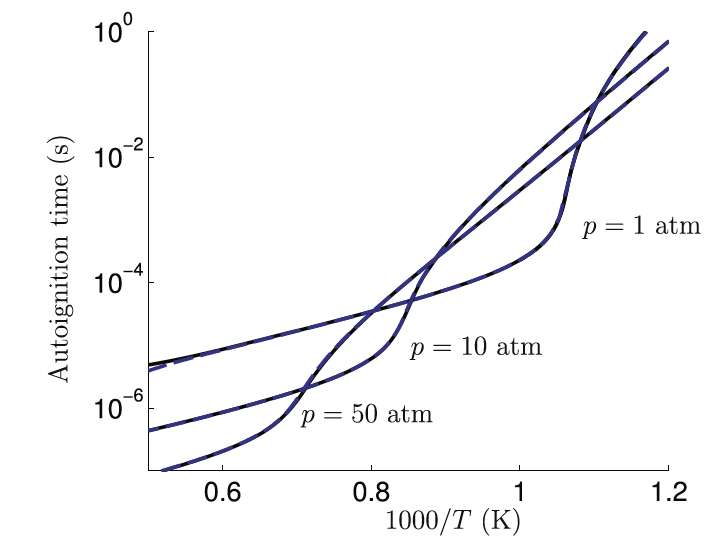
\includegraphics[width=.4\textwidth]{figures/autoignition.png}
%\end{multicols}
%\end{frame}

%\begin{frame}\frametitle{\textit{Prometheus} / \textit{mirgecom} wishlist}
%\begin{itemize}
%   \item get\_species\_index(species\_name) - useful for coding the interface/wrappers
%   \item get\_species\_names - for I/O, viz/analysis
%\end{itemize}           
%\end{frame}
%
\begin{frame}\frametitle{Demo}
Isentropic vortex after Hesthaven \& Warburton, Section 6.6 (\texttt{mirgecom/initializers.py Vortex2D}):\\
\vspace{.2in}
$\vec{v}(r) = \vec{v}_0 + \frac{\beta{e}^{(1 - r^2)}}{2\pi}\langle{y}_0 - y,x - x_0\rangle$\\
$\rho(r) = ( 1 - (\frac{\gamma-1}{16\gamma\pi^{2}})\beta^{2}{e}^{2(1-r^{2})})^{\frac{1}{\gamma-1}}$\\
$p = \rho^{\gamma}$\\
%\end{math}
where $r = \vec{r} - \vec{r}_0 - \vec{v}_0{t}$, with $r_0 = (5, 0), \beta=5, \gamma=1.4$, and $\vec{v}_0 = (1,1)$.\\
\vspace{.2in}
Box domain [0, 10]x[-5, 5], advanced with RK4, and exact BCs (i.e. prescribed $\mathbf{Q}^{+}$ on domain boundaries).\\
\vspace{.2in}
Driver: \texttt{examples/vortex-mpi.py}
%\vspace*{0.35in}
%\begin{center}
%\cPI{\huge Demo}
%\end{center}
\end{frame}

\begin{frame}\frametitle{Next steps}
\begin{multicols}{2}
\begin{itemize}
\item For everyone:
\begin{itemize}
\item Go try it! \href{https://github.com/illinois-ceesd/mirgecom}{(\textcolor{blue}{https://github.com/illinois-ceesd/mirgecom})}
\item Contribute: Fork + Pull Request 
\end{itemize}
\item For \textit{mirgecom}:
\begin{itemize}
\item Restart
\item Ideal mixtures + \textit{Prometheus}
\item Chemistry
\item Navier-Stokes
\item Shock handling
\end{itemize}
\end{itemize}

\end{multicols}
  \ifmovies{
    \begin{center}
      \movie[autostart,loop,showcontrols=false,width=\textwidth]{
        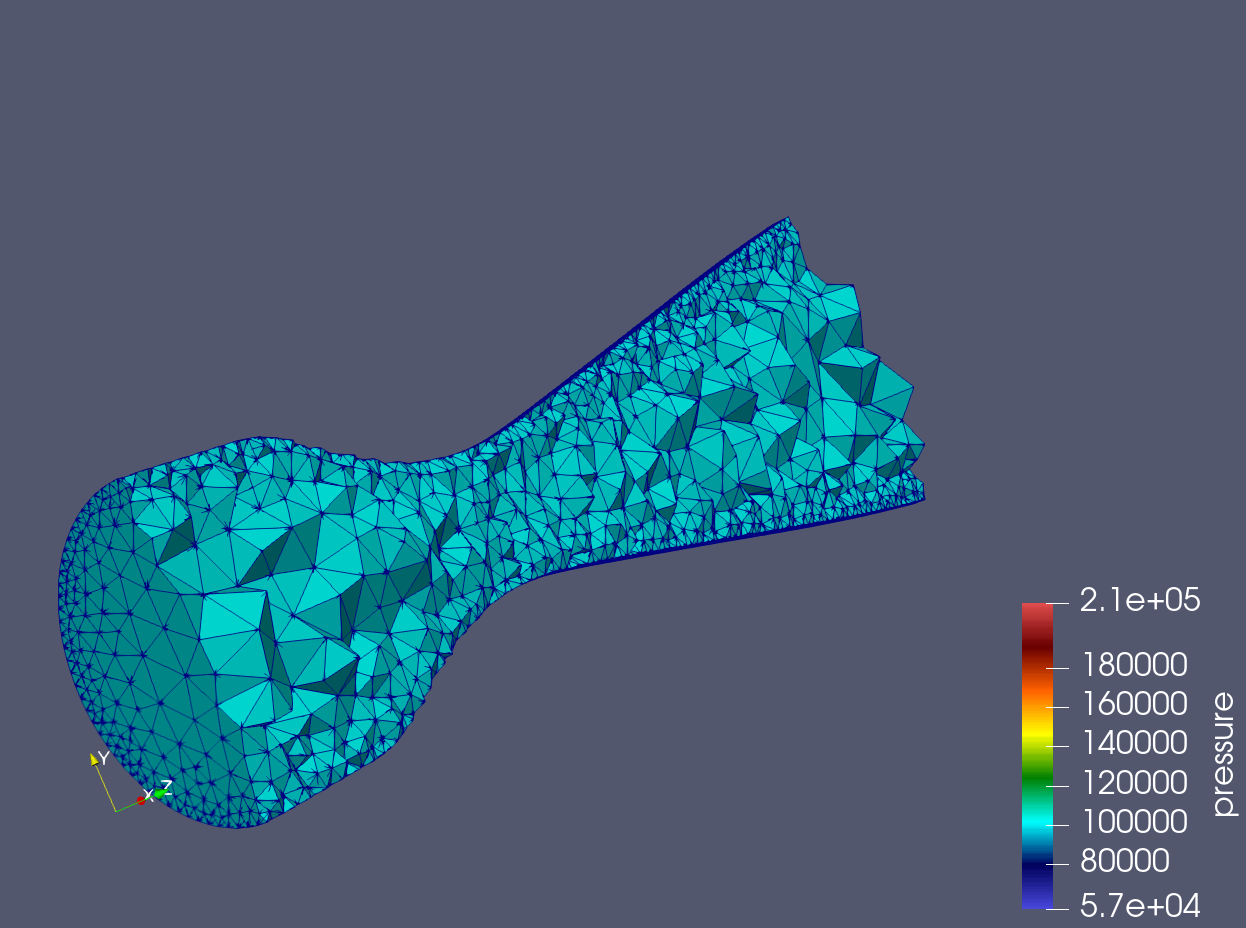
\includegraphics[width=.5\textwidth]{figures/Y1Nozzle-0.png}}{figures/Y1Nozzle3.mov}
    \end{center}
  }\else{
    \begin{center}
      \includegraphics[width=.5\textwidth]{figures/Y1Nozzle-2400.png}
    \end{center}
  }\fi
  \begin{center}
  [Y0/Y1 geometry (~1M Tetrahedra) from Matt Smith]
  \end{center}
%\begin{center}
%\includegraphics[width=1.0\textwidth]{Figures/multi-physics-crop.pdf}
%  \textcolor{red}{TODO: Y1 flow}
%\end{center}
%\begin{multicols}{2}
%  \begin{itemize}
%  \item Initial Y1 mesh, 1M tetrahedra
%  \item Inviscid, single gas
%  \item Subsonic injection
%  \item GPU and CPU access through \textit{PyOpenCL}
%  \end{itemize}
\end{frame}

\begin{frame}\frametitle{}

\vspace*{0.2in}

\begin{center}

%
\includegraphics[width=0.5\textwidth]{Figures/ceesd-logo-2.pdf}
\vspace*{0.35in}
\cPI{\huge Questions?}
%\newline
%\newline
\vspace{5mm}
\begin{minipage}{0.8\textwidth}
This material is based in part upon work supported by the Department of Energy, National Nuclear Security Administration, under Award Number \textit{DE-NA0003963}.
\end{minipage}
\end{center}
\end{frame}

%\begin{frame}\frametitle{Reactive Flow Equations}
%  \begin{align*}
%    \pop{\rho}{t} + \Grad\cdot\pp{ \rho \bvec{u} } &= 0 \\
%    \pop{ \rho\bvec{u} }{t} + \Grad\cdot\pp{ \rho \bvec{u}\bvec{u} } &= -\Grad p + \Grad\cdot\bvec{\tau} \\
%    \pop{ \rho E }{t} + \Grad\cdot\pp{ \rho E \bvec{u} } &= -\Grad\cdot\pp{ p\bvec{u} } + \Grad\cdot\pp{ \bvec%{\tau} \cdot \bvec{u} } - \Grad\cdot\bvec{q} \\
%    \pop{\rho Y_{i}}{t} + \Grad\cdot\psq{ \rho Y_{i}\pp{ \bvec{u} + \bvec{V}_{i} } } &= W_{i}\dot{\omega}_{i},%\quad i = 1,\dots,N
%  \end{align*}
%  \begin{align*}
%    \bvec{\tau} = 2\mu\psq{ \mathbf{S} - \frac{1}{3}\pp{ \Grad\cdot\bvec{u} }\mathbf{I} }\\
%    \bvec{q} = -\kappa\Grad T + \sum_{i = 1}^{N}\rho Y_{i} h_{i}\bvec{V}_{i} \\
%    Y_{i}\bvec{V}_{i} = \frac{D_{im}W_{i}}{W}\Grad X_{i}\\
%  \end{align*}
%\end{frame}
%======================================================================

%======================================================================
%\begin{frame}\frametitle{Chemical Source Term}
%  \begin{align*}
%    \omega_{i} &= \nu_{ij}R_{j} \\
%    R_{j} &= k_{j}(T)\psq{ \prod_{m = 1}^{N}\pp{\frac{\rho Y_{m}}{W_{m}}}^{\nu_{mj}^{\prime}} - \frac{1}{K_{j}%(T)}\prod_{n = 1}^{N}\pp{\frac{\rho Y_{m}}{W_{m}}}^{\nu_{nj}^{\prime\prime}}  } \\
%    K_{j}(T) &= \pp{ \frac{p_{0}}{RT} }^{\sum_{i = 1}^{N}\nu_{ij}}\exp\psq{ -\sum_{m = 1}^{N} \frac{\nu_{mj}g_%{m}(T)}{RT} } \\
%    k_{j}(T) &= A_{j} T^{b_{j}}\exp\pp{ -\frac{E_{a,j}}{RT} } \\
%    \frac{g_{i}(T)}{RT} &= \frac{h_{i}(T)}{RT} - \frac{s_{i}}{R} \\
%    \frac{h_{i}(T)}{RT},\,\frac{s_{i}(T)}{R} &: \text{NASA polynomials}
%  \end{align*}
%\end{frame}
%======================================================================
\end{document}
